\subsubsection{Counting Convolutional Parameters}\label{sec:counting-convolutional-parameters}

Given the input depth, the kernel size, and the number of filters, \emph{\textbf{how many trainable numbers does this convolutional layer contain?}}

\highspace
For a convolutional layer with:
\begin{itemize}
    \item $C_{\text{in}}$ input channels (depth),
    \item $C_{\text{out}}$ output channels (number of filters),
    \item $K_h$ kernel height,
    \item $K_w$ kernel width,
    \item $K_h \times K_w$ kernel size,
\end{itemize}
The \textbf{number of trainable parameters} is:
\begin{equation}
    \text{Number of trainable parameters} = C_{\text{out}} \left( K_h K_w C_{\text{in}} + 1 \right)
\end{equation}
Where the $+1$ is the \textbf{bias} associated with each filter. This equation is exactly the same as the one derived on \autopageref{eq:number-of-trainable-parameters-in-a-convolutional-layer}.

\begin{figure}[!htp]
  \centering
  \resizebox{\linewidth}{!}{%
  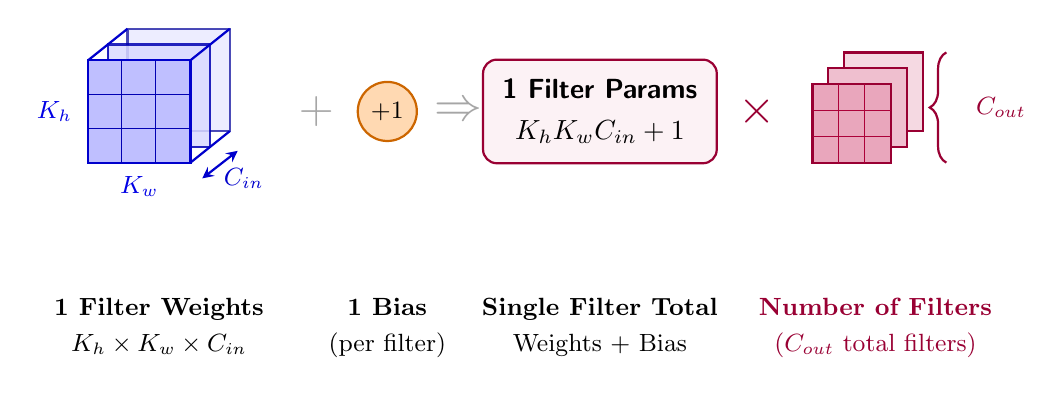
\begin{tikzpicture}[
    >=stealth,
    scale=1.0,
    font=\sffamily,
    % --- Custom Styles ---
    layerFront/.style={draw=blue!80!black, fill=blue!25, thick},
    layerMid/.style={draw=blue!70!black, fill=blue!15, thick, opacity=0.85},
    layerBack/.style={draw=blue!60!black, fill=blue!10, thick, opacity=0.7},
    biasStyle/.style={circle, draw=orange!80!black, fill=orange!30, thick, inner sep=2pt, font=\small\bfseries},
    boxStyle/.style={draw=purple!80!black, fill=purple!5, rounded corners=5pt, thick, inner sep=7pt, align=center},
    labelStyle/.style={font=\small, align=center, text=black}
  ]

    % =========================================================
    % STEP 1: ONE 3D FILTER VOLUME (Kh x Kw x Cin)
    % =========================================================
    % Back Channel Slice
    \begin{scope}[shift={(0.5cm, 0.4cm)}]
      \draw[layerBack] (0,1.2) rectangle (1.3,2.5);
    \end{scope}
    
    % Middle Channel Slice
    \begin{scope}[shift={(0.25cm, 0.2cm)}]
      \draw[layerMid] (0,1.2) rectangle (1.3,2.5);
    \end{scope}
    
    % Front Channel Slice (3x3 Grid)
    \begin{scope}[shift={(0,1.2)}]
      \draw[layerFront] (0,0) rectangle (1.3,1.3);
      % 3x3 Grid lines
      \draw[blue!70!black, thin] (0.43,0) -- (0.43,1.3);
      \draw[blue!70!black, thin] (0.86,0) -- (0.86,1.3);
      \draw[blue!70!black, thin] (0,0.43) -- (1.3,0.43);
      \draw[blue!70!black, thin] (0,0.86) -- (1.3,0.86);
    \end{scope}

    % Outer connecting 3D edges
    \draw[blue!80!black, thick] (0,2.5) -- (0.5,2.9);
    \draw[blue!80!black, thick] (1.3,2.5) -- (1.8,2.9);
    \draw[blue!80!black, thick] (1.3,1.2) -- (1.8,1.6);

    % Dimension Annotations
    \node[anchor=north, font=\small, text=blue!90!black] at (0.65, 1.15) {$K_w$};
    \node[anchor=east, font=\small, text=blue!90!black] at (-0.08, 1.85) {$K_h$};
    
    % Cin Depth Dimension Arrow
    \draw[thick, blue!80!black, <->] (1.45, 1.0) -- (1.9, 1.35) 
      node[midway, below right, font=\small, inner sep=1pt] {$C_{\text{in}}$};

    % =========================================================
    % STEP 2: ADD BIAS (+1)
    % =========================================================
    \node[font=\LARGE\bfseries, text=gray!70] at (2.9, 1.85) {$+$};
    \node[biasStyle, minimum size=7.5mm] (bias) at (3.8, 1.85) {$+1$};

    % =========================================================
    % STEP 3: EQUALS ONE FILTER PARAMS
    % =========================================================
    \node[font=\LARGE\bfseries, text=gray!70] at (4.7, 1.85) {$\Rightarrow$};

    \node[boxStyle] (perFilterBox) at (6.5, 1.85) {
      \textbf{1 Filter Params}\\[3pt]
      $\boxed{K_h K_w C_{\text{in}} + 1}$
    };

    % =========================================================
    % STEP 4: MULTIPLY BY C_out (STACK OF FILTERS)
    % =========================================================
    \node[font=\LARGE\bfseries, text=purple!80!black] at (8.5, 1.85) {$\times$};

    % Stack of Cout Filters
    \begin{scope}[shift={(9.2cm, 1.2cm)}]
      \draw[draw=purple!80!black, fill=purple!15, thick] (0.4, 0.4) rectangle (1.4, 1.4);
      \draw[draw=purple!80!black, fill=purple!25, thick] (0.2, 0.2) rectangle (1.2, 1.2);
      \draw[draw=purple!80!black, fill=purple!35, thick] (0, 0) rectangle (1.0, 1.0);
      \draw[purple!90!black, thin] (0.33,0) -- (0.33,1.0);
      \draw[purple!90!black, thin] (0.66,0) -- (0.66,1.0);
      \draw[purple!90!black, thin] (0,0.33) -- (1.0,0.33);
      \draw[purple!90!black, thin] (0,0.66) -- (1.0,0.66);
    \end{scope}

    % Curly Brace for Cout Stack
    \draw[decorate, decoration={brace, amplitude=6pt}, thick, purple!80!black]
      (10.9, 1.2) -- (10.9, 2.6)
      node[midway, right=7pt, font=\small\bfseries, text=purple!80!black] {$C_{\text{out}}$};

    % =========================================================
    % UNIFIED CAPTION BASELINE
    % =========================================================
    \node[labelStyle, anchor=north] at (0.9, -0.4) {
      \textbf{1 Filter Weights}\\[2pt] 
      $K_h \times K_w \times C_{\text{in}}$
    };

    \node[labelStyle, anchor=north] at (3.8, -0.4) {
      \textbf{1 Bias}\\[2pt] 
      (per filter)
    };

    \node[labelStyle, anchor=north] at (6.5, -0.4) {
      \textbf{Single Filter Total}\\[2pt] 
      Weights + Bias
    };

    \node[labelStyle, anchor=north, text=purple!80!black] at (10.0, -0.4) {
      \textbf{Number of Filters}\\[2pt] 
      ($C_{\text{out}}$ total filters)
    };

  \end{tikzpicture}%
  }
  \caption{Derivation of the number of trainable parameters in a convolutional layer. Each filter spans the complete input depth and therefore contains $K_h K_w C_{\text{in}}$ weights, plus one bias. Since the layer contains $C_{\text{out}}$ independent filters, the total number of trainable parameters is $C_{\text{out}} \left( K_h K_w C_{\text{in}} + 1 \right)$.}
  \label{fig:counting-convolutional-parameters}
\end{figure}

\highspace
\begin{flushleft}
    \textcolor{Green3}{\faIcon{tools} \textbf{Build the formula}}
\end{flushleft}
The easiest way to understand it is to forget the full formula at first. Let's suppose we have \textbf{one filter}. Because a \textbf{filter} spans the entire input depth, its \textbf{full shape} is:
\begin{equation*}
    \text{Filter shape} = K_h \times K_w \times C_{\text{in}}
\end{equation*}
Therefore, one filter has $K_h K_w C_{\text{in}}$ weights. Then it also owns one bias, so the \textbf{total number of trainable parameters for one filter} is:
\begin{equation*}
    \text{Trainable parameters for one filter} = K_h K_w C_{\text{in}} + 1
\end{equation*}
Now if the layer has $C_{\text{out}}$ filters, we simply multiply by the number of filters:
\begin{equation*}
    \text{Trainable parameters for the layer} = C_{\text{out}} \left( K_h K_w C_{\text{in}} + 1 \right)
\end{equation*}
That is the entire derivation.

\highspace
\begin{examplebox}[: RGB Input]
    Suppose $C_{\text{in}} = 3$ (RGB input), with $32$ filters of size $3 \times 3$. One filter has $3 \cdot 3 \cdot 3 = 27$ weights, plus one bias, for a total of $28$ trainable parameters. Now multiply by the number of filters: $28 \cdot 32 = 896$ trainable parameters in total. So the formula is:
    \begin{equation*}
        \text{Trainable parameters} = 32 \left( 3 \cdot 3 \cdot 3 + 1 \right) = 32 \left( 27 + 1 \right) = 32 \cdot 28 = 896
    \end{equation*}
\end{examplebox}

\highspace
\begin{examplebox}[: Deeper Convolutional Layer]
    Suppose the input is not RGB anymore, but the output of a previous convolutional layer which produces $64$ feature maps. Therefore, $C_{\text{in}} = 64$, and we still have $32$ filters of size $3 \times 3$. Then one filter has $3 \cdot 3 \cdot 64 = 576$ weights, plus one bias, for a total of $577$ trainable parameters. Now multiply by the number of filters: $577 \cdot 32 = 18464$ trainable parameters in total. So the formula is:
    \begin{equation*}
        \text{Trainable params} = 32 \left( 3 \cdot 3 \cdot 64 + 1 \right) = 32 \left( 576 + 1 \right) = 32 \cdot 577 = 18464
    \end{equation*}
    So even though the kernel size and number of filters are the same as before, the \textbf{layer} has many \textbf{more parameters} because the \textbf{input depth is larger}.

    This is exactly the point emphasized earlier when we noted that layers with the same apparent hyperparameters may have different parameter counts depending on where they occur in the network.
\end{examplebox}
\noindent
\textcolor{Green3}{\faIcon{question-circle} \textbf{What does not appear in the formula?}} The input spatial dimensions $H_{\text{in}}$ and $W_{\text{in}}$ do \textbf{not} appear in the parameter-count formula. This is because the same filter is reused at every spatial position. Whether the input is $32 \times 32 \times 3$ or $1024 \times 1024 \times 3$, a layer with $32$ filters of size $3 \times 3$ will always have $896$ trainable parameters. \hl{The input spatial dimensions only affect the output spatial dimensions, not the number of trainable parameters.} This is the consequence of the \textbf{weight sharing} property of convolutional layers.

\highspace
\begin{takeawaysbox}
    \begin{itemize}
        \item Each filter contains $K_h K_w C_{\text{in}}$ weights because it spans the complete input depth.
        \item Each filter has one bias.
        \item There are $C_{\text{out}}$ filters, so the total parameters count is:
        \begin{equation*}
            C_{\text{out}} \left( K_h K_w C_{\text{in}} + 1 \right)
        \end{equation*}
        \item Input height and width do not affect the number of trainable parameters because the same filter is reused spatially.
    \end{itemize}
\end{takeawaysbox}